\documentclass[UTF8, xcolor=table]{beamer}
\usepackage[BoldFont,SlantFont]{xeCJK}
\setCJKmainfont[BoldFont={Adobe Heiti Std},ItalicFont={Adobe Kaiti Std}]{AdobeSongStd-Light}
% \setCJKmainfont[BoldFont={Adobe Heiti Std},ItalicFont={Adobe Kaiti Std}]{SimSum} %Windows先编译使用这个字体

\usepackage{latexsym,amssymb,amsmath,amsbsy,amsopn,amstext,xcolor,multicol}
\usepackage{graphicx,wrapfig,fancybox}
\usepackage{pgf,pgfarrows,pgfnodes,pgfautomata,pgfheaps,pgfshade}
\usepackage{thubeamer}
\usepackage[backend=bibtex,sorting=none]{biblatex} % [参考文献格式](https://www.sharelatex.com/blog/2013/07/31/getting-started-with-biblatex.html) %mac IEEE not found
\usepackage{array}
\usepackage{bm}
\usepackage{caption}
\RequirePackage[font=footnotesize]{subcaption}
\usepackage{multirow}
\usepackage{booktabs}
\usepackage{tikz}
\usepackage{tikzscale}
\usepackage{animate}

\defbibheading{bibliography}[\bibname]{} %avoid printbibliography 自动生成目录
\addbibresource{../main.bib}
\setbeamertemplate{bibliography item}[text] 

\usepackage{boxedminipage} %for: bvh border
\def\fourgraphicswidth{0.35} %0.3\textwidth

\usepackage{algorithm} %%format of the algorithm
\usepackage{algpseudocode}
\floatname{algorithm}{算法}
\renewcommand{\algorithmicrequire}{\textbf{输入:}} % Use Input in the format of Algorithm
\renewcommand{\algorithmicensure}{\textbf{输出:}} % UseOutput in the format of Algorithm
\algrenewcommand{\algorithmiccomment}[1]{ $//$ #1}

\usepackage{listings}
\renewcommand\lstlistingname{代码}
\renewcommand\lstlistlistingname{代码}

\lstset{framexleftmargin=1.4em,
        xleftmargin=1.8em,
        basicstyle=\ttfamily\small,
        %frame=shadowbox, numberstyle=\tiny, breaklines=true,
        frame=single,
        numberstyle=\tiny, breaklines=true,
        keywordstyle=\color{blue!70}\bfseries,
        %commentstyle=\color{red!50!green!50!blue!50},
        rulesepcolor=\color{red!20!green!20!blue!20},
        numbers=none,fontadjust=true}
\lstdefinelanguage{shader}{morekeywords={uniform, layout, uniform, vec2, vec3, vec4, in, out, gl_Position, dot, flat, int ,float, gl_VertexID, xyz, w, x, y, z, location, version, sampler2DRect, bgr, gl_FragData, texture2DRect, gl_TexCoord,for,xy},morecomment=[l]{//}}

\begin{document}

\setbeamerfont{footnote}{size=\tiny}
\setbeamerfont{caption}{size=\scriptsize}
\setbeamertemplate{caption}[numbered]
\setbeamerfont{subsection in toc}{size=\footnotesize}
\renewcommand*{\bibfont}{\footnotesize}

\graphicspath{{../}}

\title[融合长短记忆神经网络与卷积特征学习的图像语义分割]{中山大学本科毕业论文演示文稿非正式模版}
\author[陈冠英]{}%{(申请中山大学工学学士学位论文答辩报告)\\ \vskip 20pt 学~~~~~~生:陈~冠~英}
\institute[中山大学~电子信息与工程学院~\&~自动化]{}%{\small \vskip 38pt 电子信息与工程学院~自动化}
\date{} %{\small \vskip -17pt二〇一六年五月}

%% make title %%
\frame{
	\titlepage
	\vspace{-23mm}
	\begin{figure}[h]
		\centering
		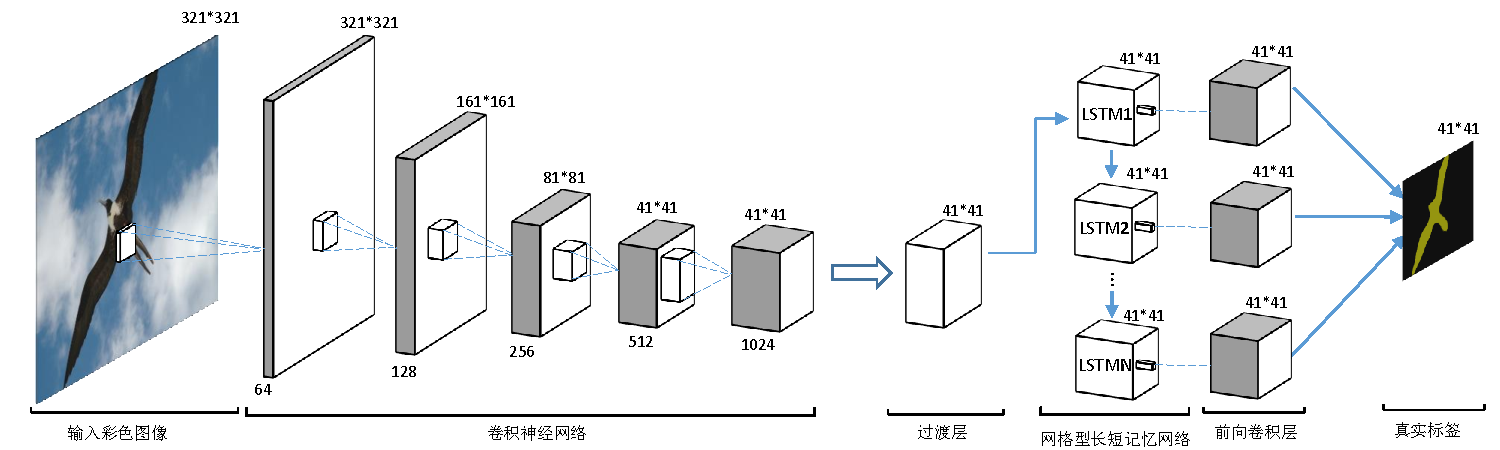
\includegraphics[width=\textwidth]{image/illustration/networkstructure.pdf}
	\end{figure}
}

\frame {
	\frametitle{目录}
	%\begin{multicols}{2}
	\tableofcontents[sections={<1-7>}]
}

\section{引言}
\frame
{
  \frametitle{\secname~ }
  \begin{block}{选题背景与意义}
	  是什么,为什么?
  \end{block}
  \begin{block}{国内外研究现状}
	  主流方法是什么?
  \end{block}
  \begin{block}{本文的工作}
	  我提出的方法是什么,有什么不同?
  \end{block}
}

\subsection*{选题背景与意义}
\frame{
  \frametitle{图像语义分割问题的定义}
  \begin{block}{}
	图像语义分割 (Semantic Image Segmentation) 是根据物体类别把图像分成若干个有意义的区域,并为不同的区域标注其所属标签的视觉任务。
  \end{block}
\begin{figure}%文中的Grid-LSTM模型做的语义图像分割的例子
	\centering
	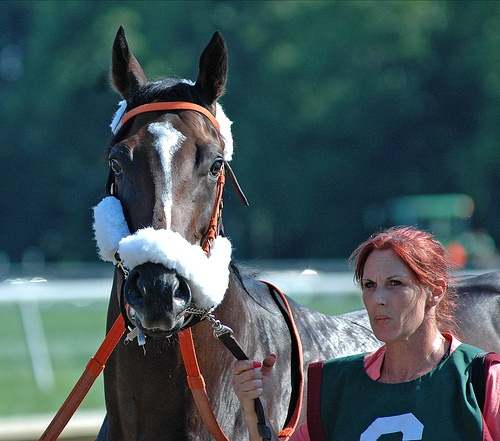
\includegraphics[width=.2\textwidth,height=.15\textwidth]{image/example/2007_000799.jpg}
	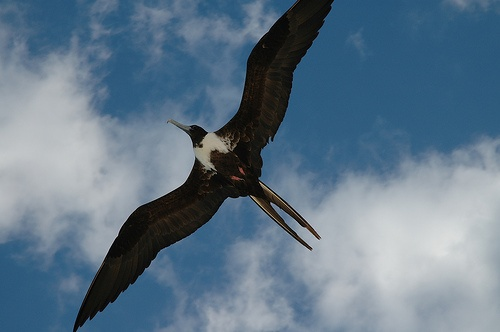
\includegraphics[width=.2\textwidth,height=.15\textwidth]{image/example/2007_002094.jpg}
	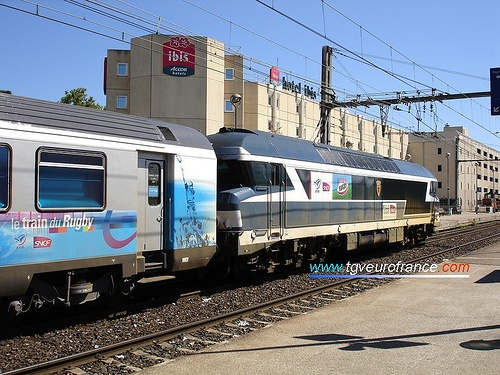
\includegraphics[width=.2\textwidth,height=.15\textwidth]{image/example/2007_004483.jpg}
	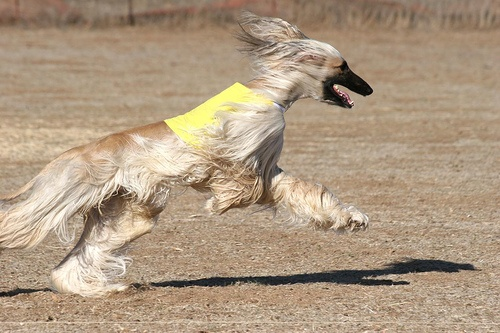
\includegraphics[width=.2\textwidth,height=.15\textwidth]{image/example/2007_003194.jpg}
	\\
	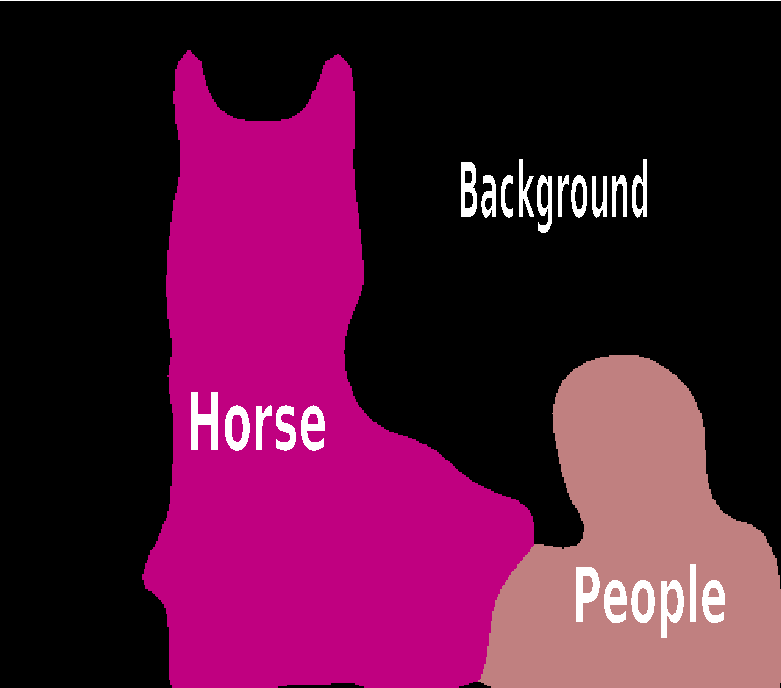
\includegraphics[width=.2\textwidth,height=.15\textwidth]{image/example/2007_000799.pdf}
	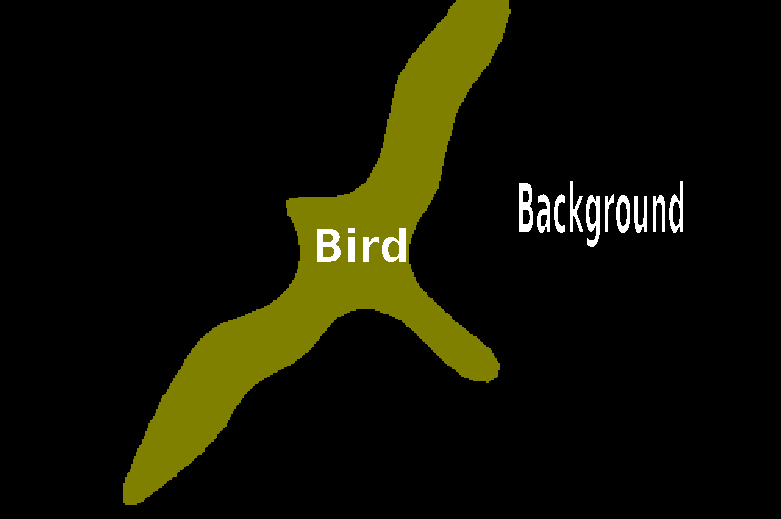
\includegraphics[width=.2\textwidth,height=.15\textwidth]{image/example/2007_002094.pdf}
	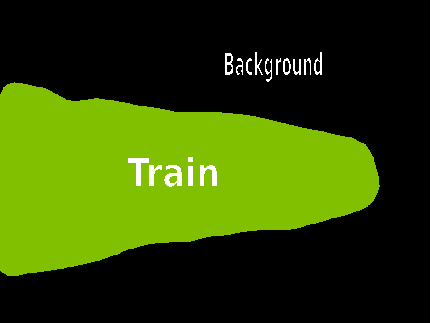
\includegraphics[width=.2\textwidth,height=.15\textwidth]{image/example/2007_004483.pdf}
	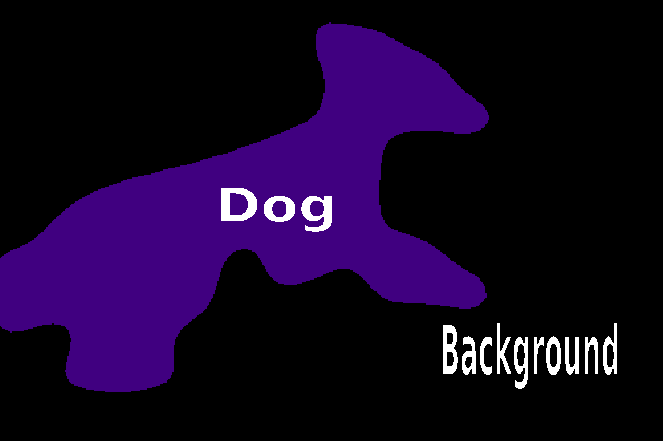
\includegraphics[width=.2\textwidth,height=.15\textwidth]{image/example/2007_003194.pdf}
	\caption[语义图像分割的例子]{本文模型在VOC 2012验证集上的语义图像分割例子}
	\label{fig:example1}
\end{figure}
}

\frame{
   \begin{block}{选题的背景}
   \begin{itemize}
	\item 手工设计特征的局限性(SIFT, HOG)
	\item 深度学习技术的兴起
		\begin{itemize}
			\item 基于GPU的并行化计算 
			\item 大型训练集的标注 
		\end{itemize}
	\item 大数据与智能时代正在来临
   \end{itemize}
   \end{block}

   \begin{block}{选题的意义}
	\begin{itemize}
		\item[\dag] 图像语义分割解决了图像里面有什么,物体的形状与位置的问题
   \end{itemize}
   \vspace{-1em}
   \begin{multicols}{2}
   \begin{itemize}
	\item 图像检索
	\item 图像编辑
	\item 现实增强
	\item 机器导航
   \end{itemize}
   \end{multicols}
   \end{block}
   \}
}
\subsection*{国内外研究现状}

\frame{
	\frametitle{主流方法中的代表性工作}
	\begin{columns}[t]
		\column{.5\textwidth}
		\centering
		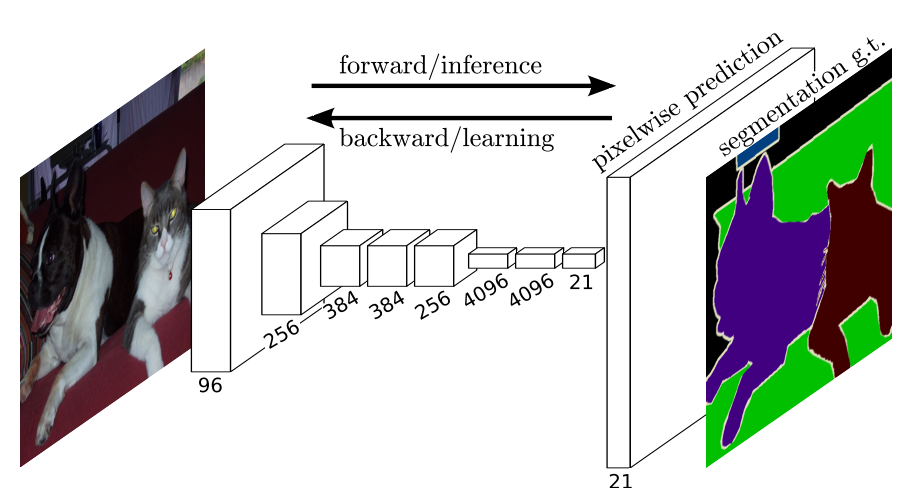
\includegraphics[width=\textwidth]{figures/FCN} \\
		\makebox[0.5\textwidth]{\tiny a. 全卷积网络[Long et al, CVPR 2015]} \\
		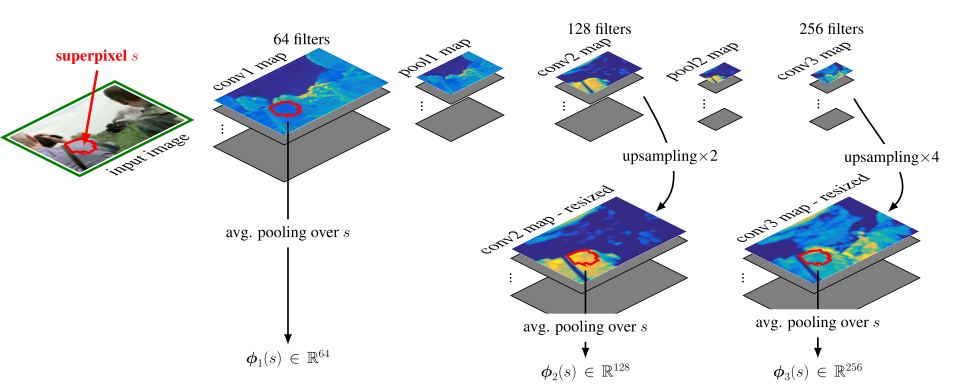
\includegraphics[width=\textwidth]{figures/zoom-out} \\
		\makebox[0.5\textwidth]{\tiny c. 卷积网络+高低层次特征融合[Mostajabi et al, CVPR 2015]} 

		\column{.5\textwidth}
		\centering
		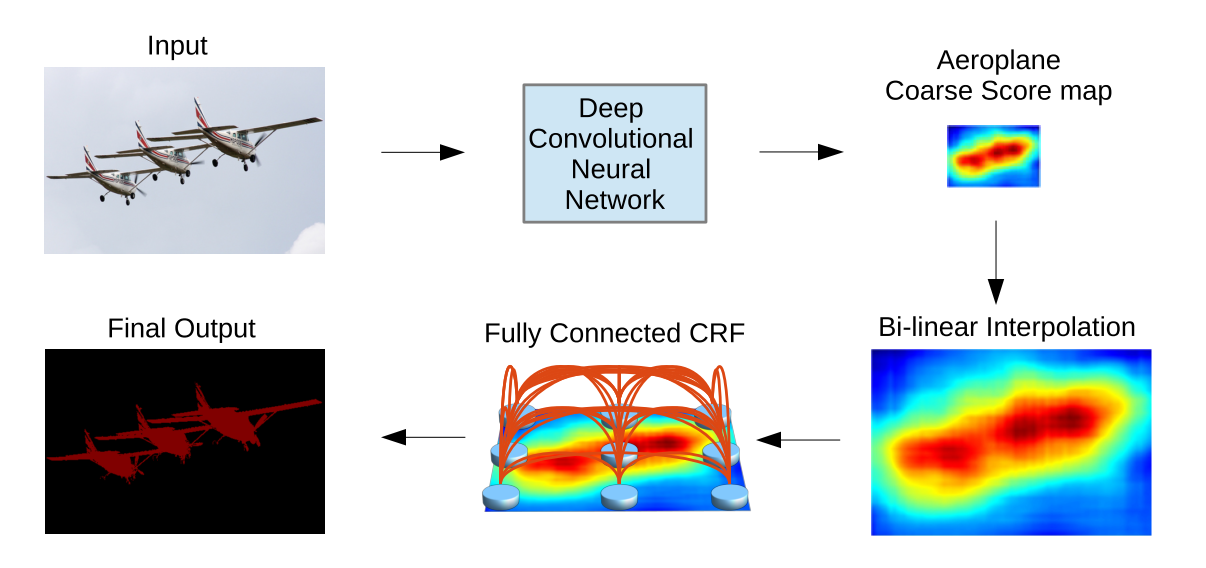
\includegraphics[width=\textwidth]{figures/Deeplab} \\
		\makebox[0.5\textwidth]{\tiny b. 全卷积网络+概率图模型[Chen et al, ICLR 2015]} \\
		\vspace{0.8em}
		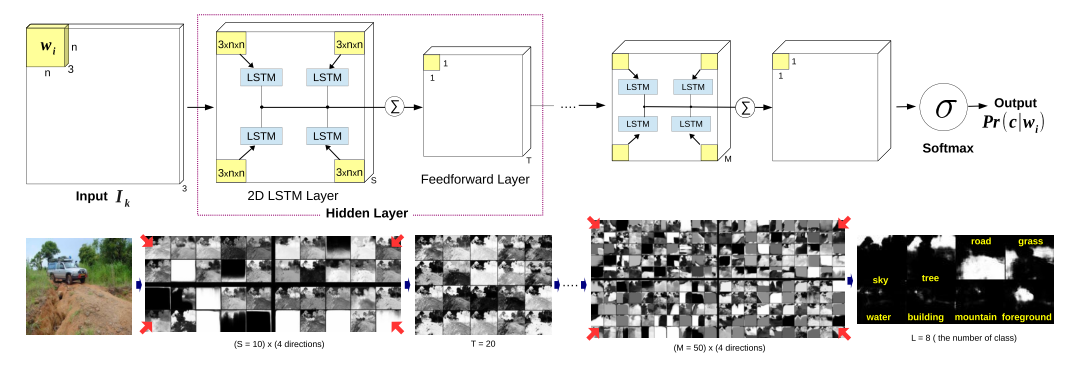
\includegraphics[width=\textwidth]{figures/LSTM} \\
		\makebox[0.5\textwidth]{\tiny d. 二维长短记忆网络[Byeon et al, CVPR, 2015]}
	\end{columns}
}
\subsection*{本文的工作}
\frame{
	\vspace{-0.6em}
	\begin{figure}[h]
		\centering
		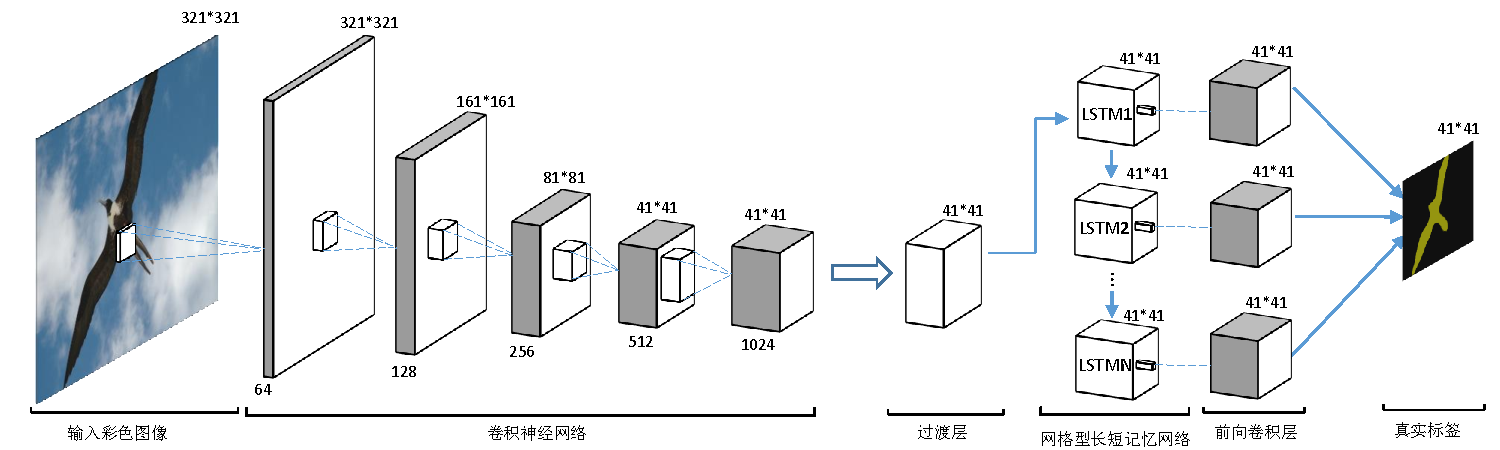
\includegraphics[width=\textwidth]{image/illustration/networkstructure.pdf}
		\caption{网络整体结构图}
	\end{figure}
	\vspace{-1.2em}
	\begin{block}{目标与思路}
		\footnotesize
	\begin{itemize}
		\item 充分利用全卷积网络强大的特征学习能力
		\item 借助长短记忆网络对特征整体与局部建模的良好能力
		\item 使用随机梯度下降法进行端到端的训练
		\item 在主流数据集验证模型有效性
	\end{itemize}
	\end{block}
}


\section{深度神经网络}
\frame
{
  \frametitle{\secname~ }
  \begin{block}{前馈神经网络}
	  传统的人工神经网络
  \end{block}
  \begin{block}{卷积神经网络}
	  目前最为流行的,广泛应用于视觉任务的神经网络
  \end{block}
  \begin{block}{长短记忆网络}
	  与卷积网络相比,更适用于处理时序信号
  \end{block}
}
\subsection*{深度神经网络}
\frame{
	\frametitle{前馈神经网络结构}
    \begin{columns}[onlytextwidth]
		\begin{column}{0.5\textwidth}
			\vspace{-1.5em}
		\begin{itemize}
			\item 有向无环图的结构
			\item 输入层(数据特征)
			\item 隐含层(映射后的特征)
			\item 输出层(预测结果)
			\item 反向传播算法(训练方法)
		\end{itemize}
		\end{column}
		\begin{column}{0.5\textwidth}
		\begin{figure}[h] %structure of LSTM
			\centering
			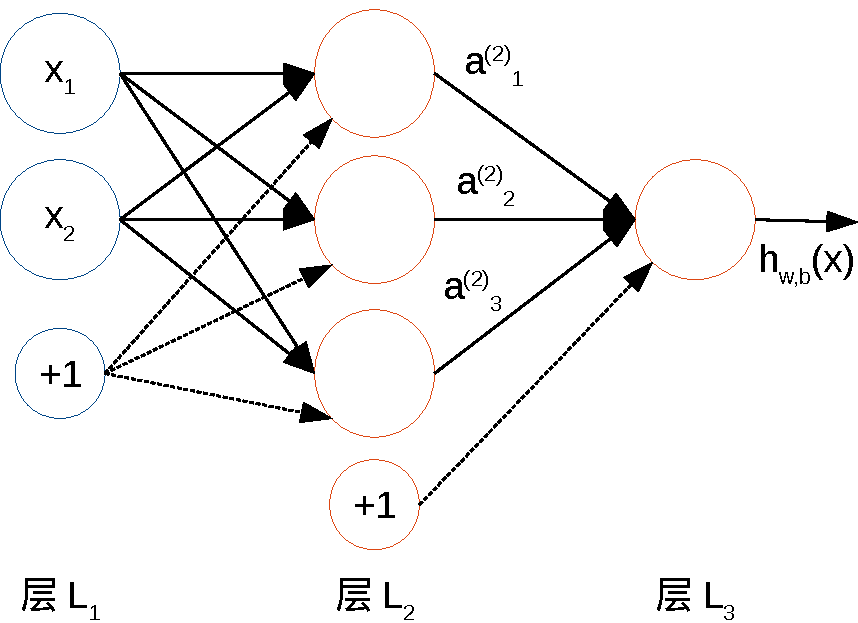
\includegraphics[width=0.9\textwidth]{image/illustration/network1.pdf}
			\caption{前馈神经网络模型示意图}
			\label{fig:lstm}
		\end{figure}
		\end{column} 
	\end{columns}
}

\frame{
   \frametitle{卷积神经网络}
   \vspace{-0.8em}
	\begin{figure}
		\centering
		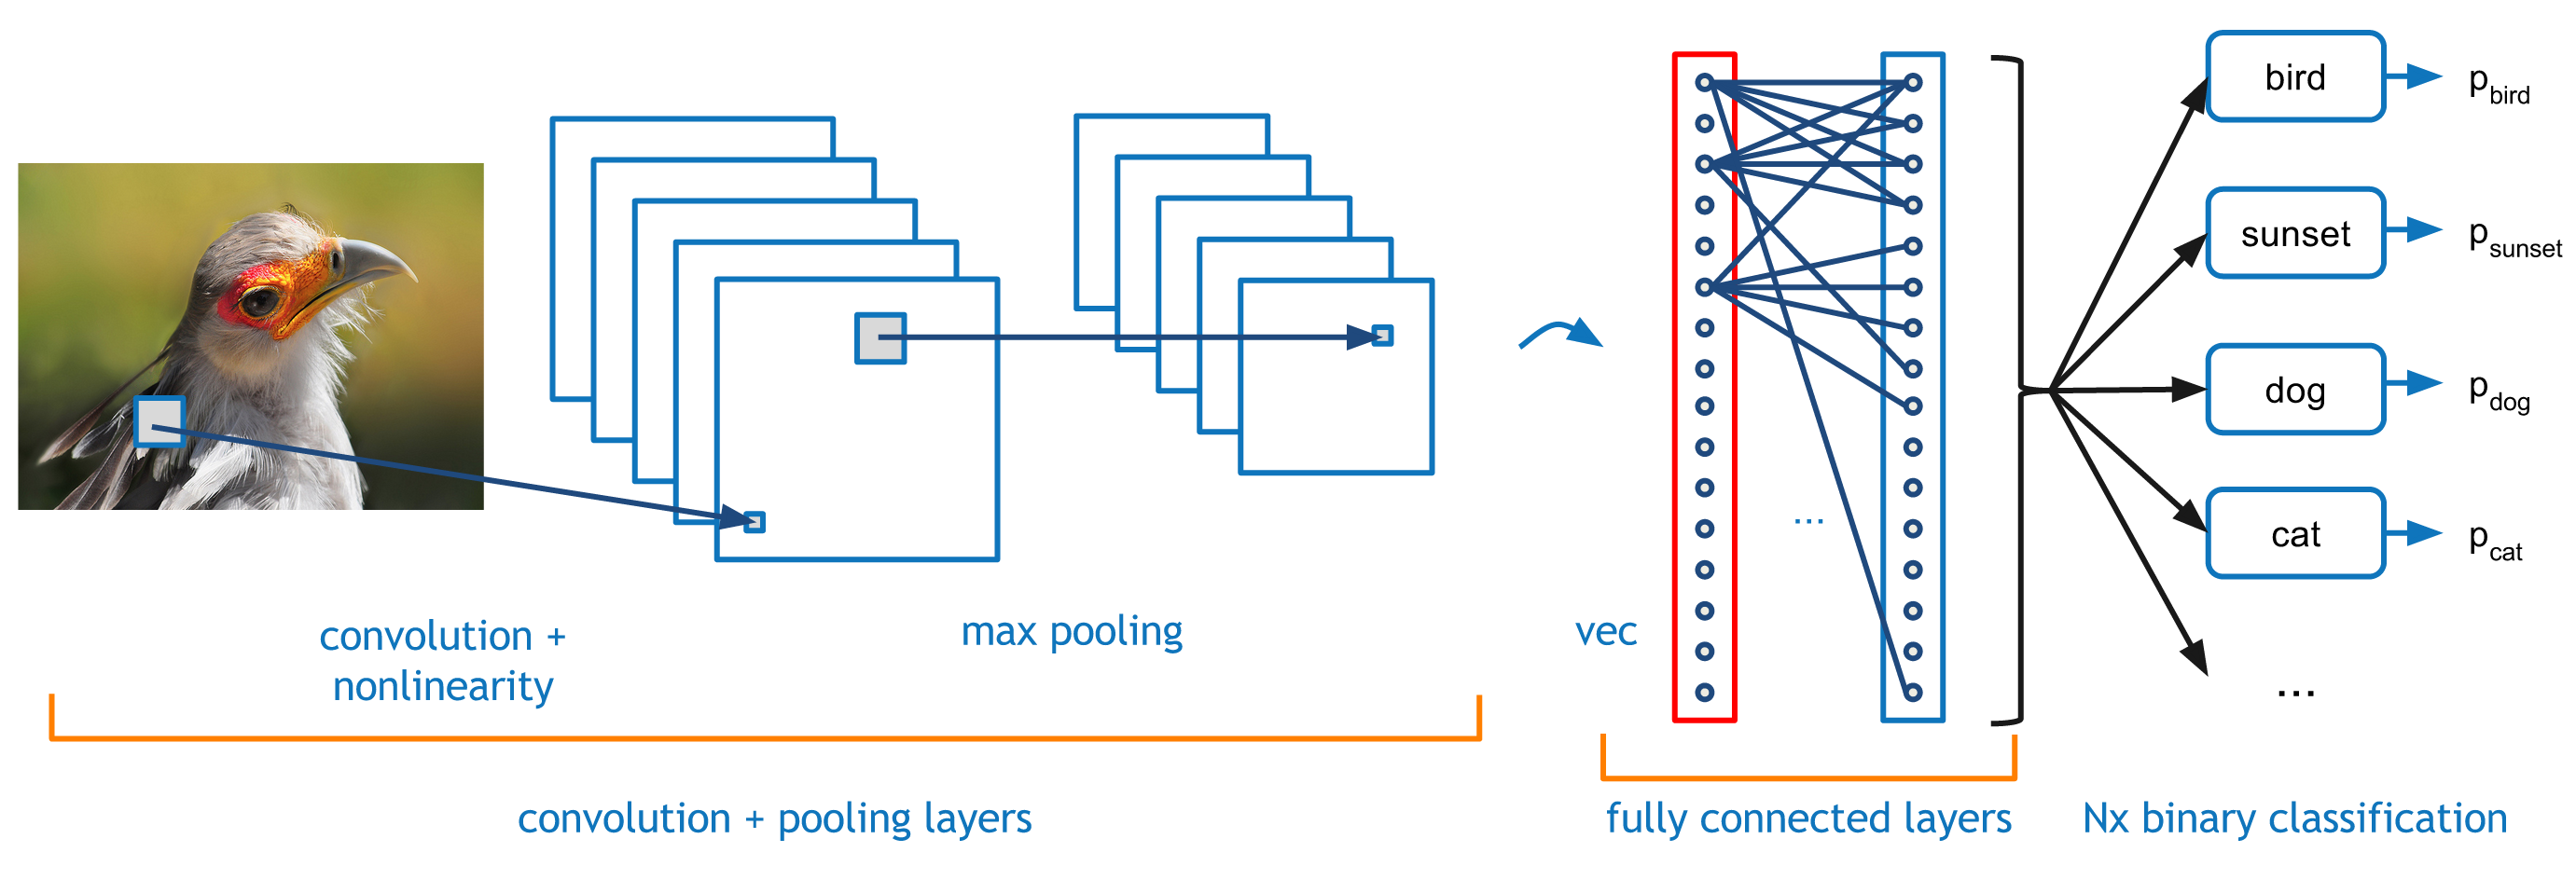
\includegraphics[width=0.8\textwidth]{figures/CNN}
		\caption{卷积网络模型示意图}
		\label{fig:network1}
	\end{figure}  
   \vspace{-0.8em}
	\begin{block}{与前馈神经网络的区别}
	\begin{itemize}
		\item 直接作用于二维图像,无需特征设计阶段
		\item 卷积层,池化层
		\item 局部感知域,权重共享
	\end{itemize}
	\end{block}
}

\frame{
	\frametitle{长短记忆网络(处理一维信号)}
	\tiny
	\vspace{-2em}
    \begin{columns}[onlytextwidth]
        \begin{column}{0.5\textwidth}
	    \begin{figure}[h] %structure of LSTM
	    	\centering
	    	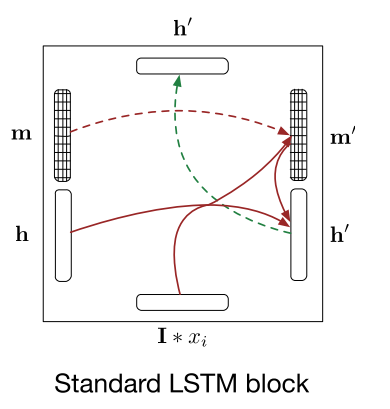
\includegraphics[width=0.6\textwidth]{figures/lstmblock1}
	    	\caption{长短记忆网络区块示意图}
	    	\label{fig:lstm}
	    \end{figure}
		\end{column} 
		%%%%%%% new column
		\begin{column}{0.5\textwidth}
			\begin{boxedminipage}{0.8\textwidth}
			\vspace{-1.5em}
			\begin{align}
				\label{eq:lstm}
				\begin{split}
				\textbf{g}^u &= \delta(\textbf{W}^u*\textbf{H}) \\
				\textbf{g}^f &= \delta(\textbf{W}^f*\textbf{H}) \\
				\textbf{g}^o &= \delta(\textbf{W}^o*\textbf{H}) \\
				\textbf{g}^c &= \mbox{tanh}(\textbf{W}^c*\textbf{H}) \\
				\textbf{m}' &= \textbf{g}^f \odot \textbf{m} + \textbf{g}^u \odot \textbf{g}^c \\
				\textbf{h}' &= \mbox{tanh}(\bf{g}^o \odot \bf{m}') \\
					\textbf{H} & = \begin{bmatrix}
					I*\textbf{x}_i \\ \textbf{h}
					\end{bmatrix}
			\end{split}
			\end{align}
		\end{boxedminipage}
		\end{column}
    \end{columns}
	
	\vspace{-1em}
	\begin{block}{缩写形式}
	\footnotesize
	\begin{equation*}
		(\textbf{h}', \textbf{m}') = \mbox{LSTM}\bigr(\textbf{H},\textbf{m},\textbf{W} \bigr)
	\end{equation*}
	其中\textbf{W}包含了四个门权值矩阵$\textbf{W}^u,\textbf{W}^f,\textbf{W}^o,\textbf{W}^c$。
	\end{block}
}

\frame{
	\frametitle{网格型长短记忆网络(处理N维信号)}
	\vspace{-1.5em}
	\begin{figure}[h]
	\centering
		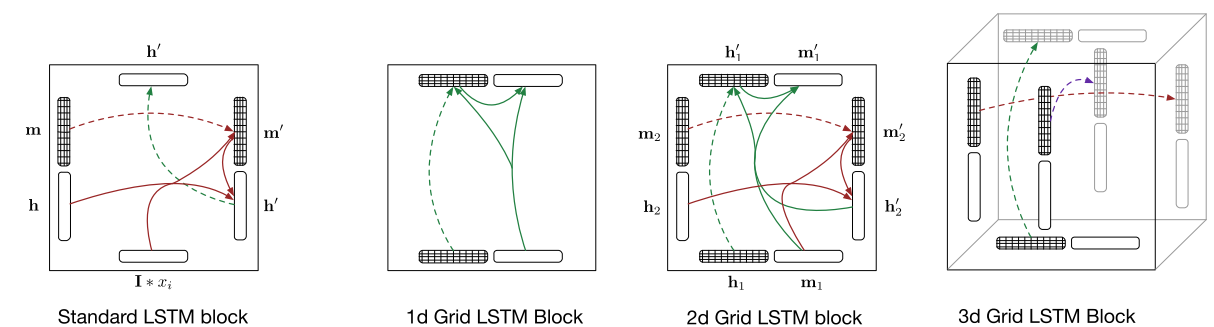
\includegraphics[width=\textwidth]{figures/gridlstm}
		\caption{网格型长短记忆网络区块示意图[Kalchbrenner et al, Grid LSTM, ICLR 2016]}
	\end{figure}
	\vspace{-2em}
	\begin{block}{网格型长短记忆网络更新过程}
	\tiny
	\begin{columns}[onlytextwidth]
		\begin{column}{0.4\textwidth}
		\vspace{-0.5em}
			\begin{equation}
				\textbf{H} = \begin{bmatrix}
					\textbf{h}_i \\ \vdots \\ \textbf{h}_N
				\end{bmatrix}
			\end{equation}
		\end{column}
		\begin{column}{0.6\textwidth}
		\vspace{-1em}
			\begin{align}
				\begin{split}
				(\textbf{h}_1', \textbf{m}_1') & =  \mbox{LSTM}(\textbf{H}, \textbf{m}_1, \textbf{W}_1) \\ &\mbox{ }\vdots \\
				(\textbf{h}_N', \textbf{m}_N') & =  \mbox{LSTM}(\textbf{H}, \textbf{m}_N, \textbf{W}_N)
				\end{split}
				\label{eq:gridlstm}
			\end{align}
		\end{column}
	\end{columns}
	\end{block}
}
\endinput

\section{网络模型结构}
\subsection*{网络模型结构}
\frame{
  \frametitle{网络整体结构}
	\begin{figure}[h]
		\centering
		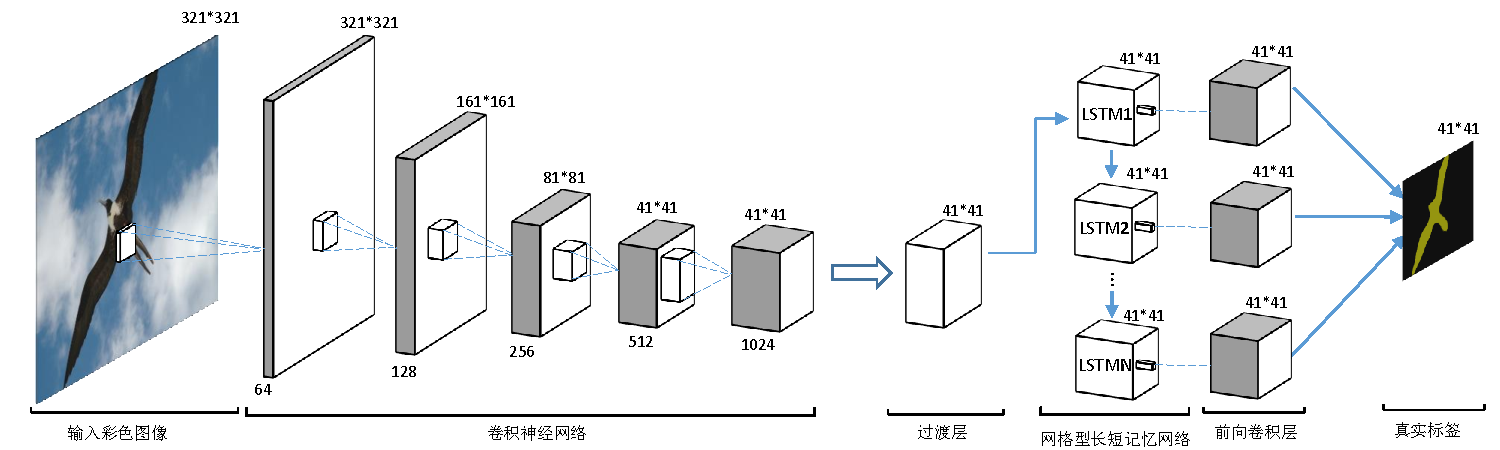
\includegraphics[width=0.9\textwidth,height=0.28\textwidth]{image/illustration/networkstructure.pdf}
		\caption{网络整体结构图}
		\label{fig:networkstructure}
	\end{figure}
	\vspace{-1em}
	\small
	\begin{block}{}
	\begin{itemize}
		\item  四个组成部分:\textbf{卷积网络部分},过渡层,\textbf{网格型长短记忆网络部分},前向卷积层
		\item 核心思想:在卷积网络后堆叠多层网格型长短记忆层
	\end{itemize}
	\end{block}
}
\frame{
	\frametitle{卷积网络部分}
	\vspace{-1em}
	\footnotesize
	\begin{block}{}
	\begin{itemize}
		\item 基于$VGG_{16}$模型\footnote{Simonyan \& Zissermanet, Very deep Convolutional Networks For Large-scale Image Recognition, ICLR 2015}, 含有16层卷积层
		\item 使用了“孔算法”,在不损失精度的情况下将模型参数减少了 6.5 倍\footnote{Chen et al, DeepLab-LargeFOV, ICLR 2015}
	\end{itemize}
	\end{block}
	\vspace{-1em}
	\begin{figure}[h]
		\centering
		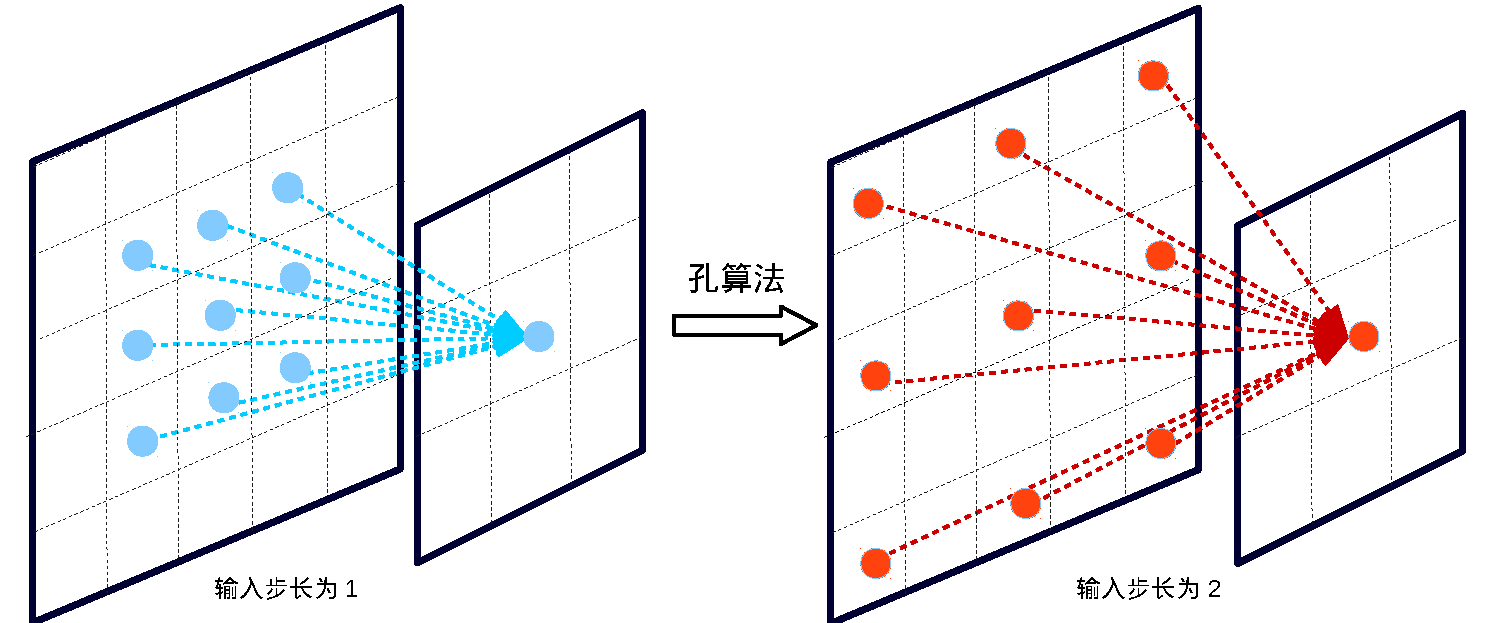
\includegraphics[width=0.7\textwidth]{image/illustration/hole.pdf}
		\caption{"孔算法"示意图}
	\end{figure}
}

\frame{
\frametitle{网格型长短记忆网络部分}
	\vspace{-1em}
    \begin{columns}%[onlytextwidth]
        \begin{column}{0.6\textwidth}
        \vspace{0.2em}
		\begin{figure}
			\centering
			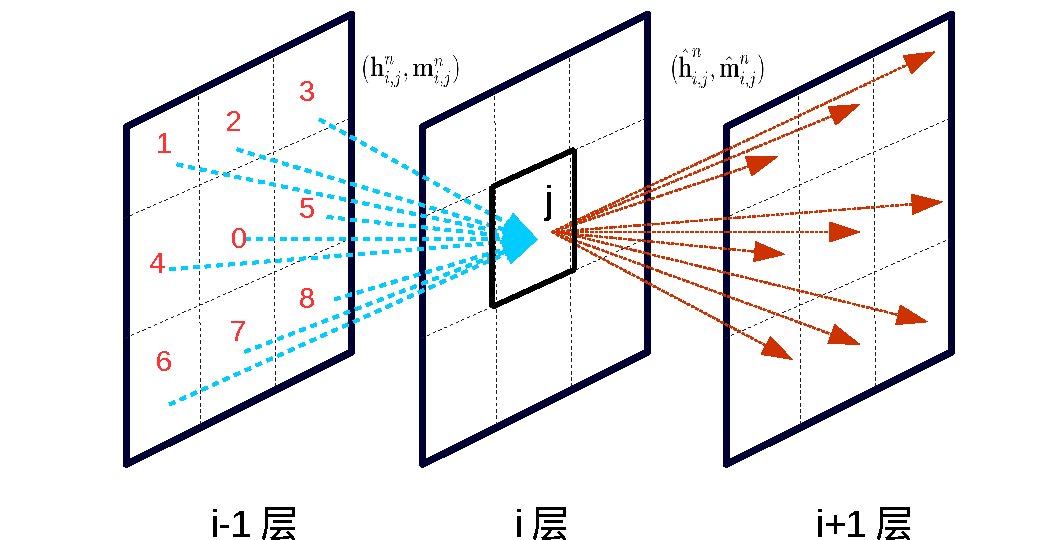
\includegraphics[width=\textwidth]{image/illustration/neighboring.pdf}
			\caption{九维网格型长短记忆网络层之间的通信示意图}
			\label{fig:neighboring}
		\end{figure}
		\end{column} 
		%%%%%%% new column
		\begin{column}{0.5\textwidth}
			\footnotesize
			\vspace{-1.5em}
			\begin{align}
				\begin{split}
				(\hat{\textbf{h}}_{i,j}^0,\hat{\textbf{m}}_{i,j}^0) &= \mbox{LSTM}(\textbf{H}_{i,j},\textbf{m}_{i,j}^0,\textbf{W}_i) \\
				(\hat{\textbf{h}}_{i,j}^1,\hat{\textbf{m}}_{i,j}^1) &= \mbox{LSTM}(\textbf{H}_{i,j},\textbf{m}_{i,j}^1,\textbf{W}_i) \\
				\vdots \\
				(\hat{\textbf{h}}_{i,j}^N,\hat{\textbf{m}}_{i,j}^N) &= \mbox{LSTM}(\textbf{H}_{i,j},\textbf{m}_{i,j}^N,\textbf{W}_i) \\
				\textbf{H}_{i,j} &= [\textbf{h}_{i,j}^0\mbox{ }\textbf{h}_{i,j}^1\mbox{ }...\mbox{ }\textbf{h}_{i,j}^N]^T
				\end{split}
			\end{align}
		\end{column}
    \end{columns}
	\footnotesize
	\vspace{-1em}
	\begin{block}{九维网格型长短记忆网络}
		\vspace{-0.7em}
		\begin{itemize}
			\item 每个位置的预测会受到上一层相邻八邻域特征的影响
			\item 随着层数的堆叠,每一位置将会有更大的感知域。
			\item 网格型长短记忆网络的层数通过实验来确定
		\end{itemize}
	\end{block}
}



\section{实验与结果}
\frame
{
  \frametitle{\secname~ }
  \begin{block}{数据集}
  \end{block}
  \begin{block}{准确率度量方式}
  \end{block}
  \begin{block}{VOC 2012实验结果}
  \end{block}
  \begin{block}{SIFT FLOW实验结果}
  \end{block}
}
\subsection*{数据集与度量方式}
\frame{
	\frametitle{Pascal VOC 2012 \& SIFT FLOW数据集}
   \vspace{-0.8em}
	\begin{figure}
		\centering
		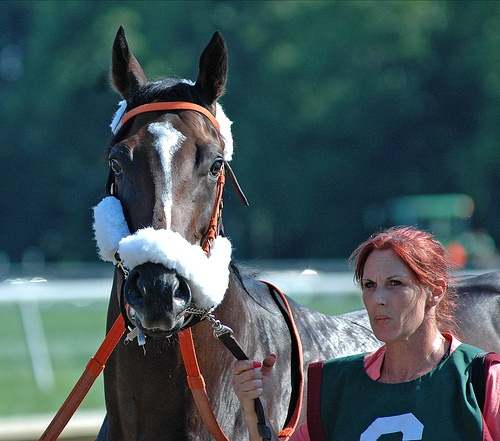
\includegraphics[width=.25\textwidth,height=.15\textwidth]{image/example/2007_000799.jpg}
		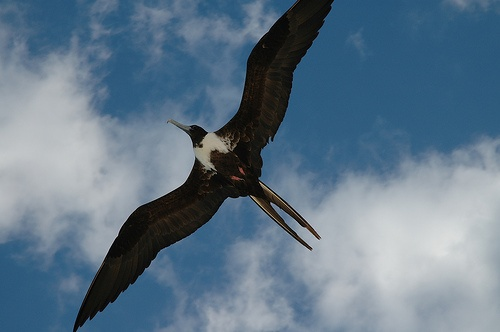
\includegraphics[width=.25\textwidth,height=.15\textwidth]{image/example/2007_002094.jpg}
		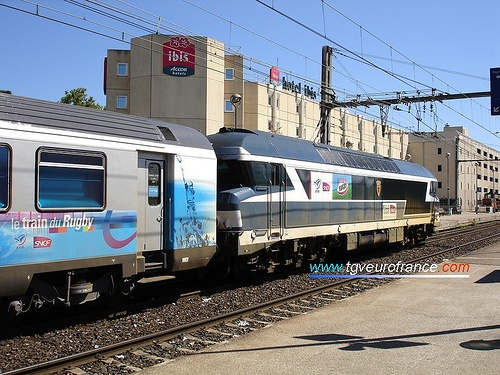
\includegraphics[width=.25\textwidth,height=.15\textwidth]{image/example/2007_004483.jpg}
		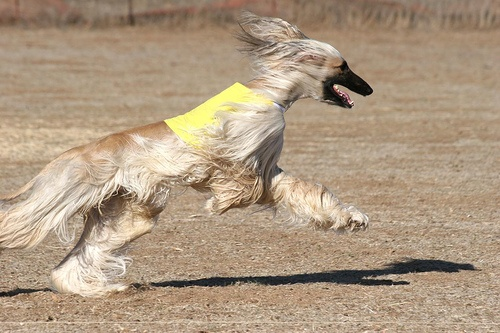
\includegraphics[width=.25\textwidth,height=.15\textwidth]{image/example/2007_003194.jpg}
		\caption{VOC 2012数据集:10582 张训练样本,1464张验证样本和1456张测试样本,21个类别}
	\end{figure}	
   \vspace{-1.8em}
	\begin{figure}[h]
		\centering
		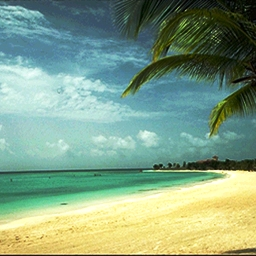
\includegraphics[width=0.25\textwidth,height=.15\textwidth]{figures/siftflow/coast_bea10.jpg}
		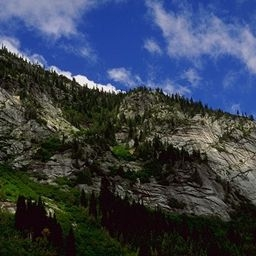
\includegraphics[width=0.25\textwidth,height=.15\textwidth]{figures/siftflow/mountain_n18058.jpg}
		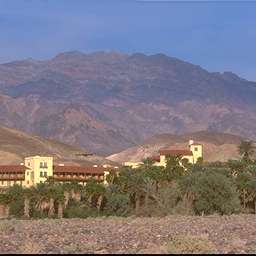
\includegraphics[width=0.25\textwidth,height=.15\textwidth]{figures/siftflow/opencountry_land732.jpg}
		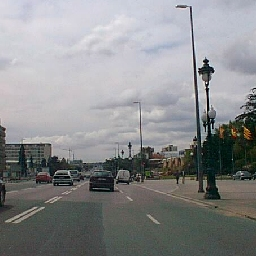
\includegraphics[width=0.25\textwidth,height=.15\textwidth]{figures/siftflow/highway_gre644.jpg}
		\caption{SIFT FLOW数据集:2488张训练样本,200张测试样本,33个类别}
		\label{fig:crop}
	\end{figure}
	\vspace{-1.2em}
	\footnotesize
	\begin{block}{图像预处理}
	\vspace{-0.5em}
	\begin{itemize}
		\item 训练时图像均缩放为321*321
		\item 随机选取训练图像,随机取镜像,数据白化
	\end{itemize}
	\end{block}
}

\frame{
   \frametitle{准确率度量方式}
   \begin{block}{}
设$n_{ij}$为真实值属于类别$i$但被分类为类别$j$的像素个数,$n_{cl}$表示有多少种不同的标签,$t_i=\sum_{j=1}^{n_{cl}}n_{ij}$为所有真实值为类别$i$的像素个数。
	\begin{align}
		\begin{split}
		\mbox{像素准确率} &= \sum_{i=1}^{n_{cl}}n_{ii} / \sum_{i=1}^{n_{cl}}t_i \\
			\mbox{平均像素准确率} &= \frac{1}{n_{cl}} \sum_{i=1}^{n_{cl}}(n_{ii}/ t_i) \\
		\mbox{Mean IU} &= \frac{1}{n_{cl}} \sum_{i=1}^{n_{cl}}\frac{n_{ii}}{t_i + \sum_j^{n_{cl}} n_{ji} - n_{ii}}
		\end{split}
	\end{align}
\end{block}
}
\subsection*{VOC 2012结果}
\frame{
   \frametitle{网格型长短记忆网络层数的选择}
   \begin{columns}
	   \begin{column}{0.5\textwidth}
			\vspace{-0.8em}
			\begin{figure}
				\centering
				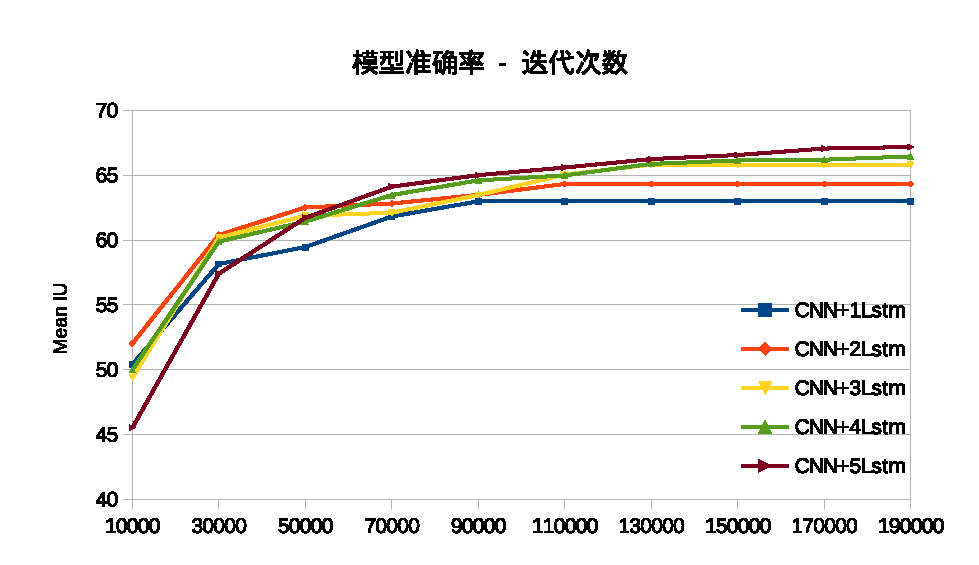
\includegraphics[width=\textwidth]{image/result/combine.eps}
				\caption{网格型长短记忆层数的不同对网络分割效果的影响方法}
				\label{fig:trainingaccuracy}
			\end{figure}
		\end{column}
	\vspace{-1.1em}
	\begin{column}{0.5\textwidth}
			\footnotesize
			\begin{itemize}
				\item[\dag] 在一定范围内增加长短记忆层数可以有效提高网络效果
				\item[\dag] 增加了5层网格型长短记忆网络之后,网络效果提升了\textbf{7.5\%}
			\end{itemize}
		\end{column}
	\end{columns}
	\vspace{-1em}
	\begin{figure}[h]
	\centering
		\makebox[0.11\textwidth]{\tiny 图像}
		\enspace
		\makebox[0.11\textwidth]{\tiny 真值}
		\enspace
		\makebox[0.11\textwidth]{\tiny CNN+5LSTM\textbf{1}}
		\enspace\thinspace
		\makebox[0.11\textwidth]{\tiny CNN+5LSTM\textbf{2}}
		\enspace\thinspace
		\makebox[0.11\textwidth]{\tiny CNN+5LSTM\textbf{3}}
		\enspace\thinspace
		\makebox[0.11\textwidth]{\tiny CNN+5LSTM\textbf{4}}
		\enspace\thinspace
		\makebox[0.11\textwidth]{\tiny CNN+5LSTM\textbf{5}}\\
		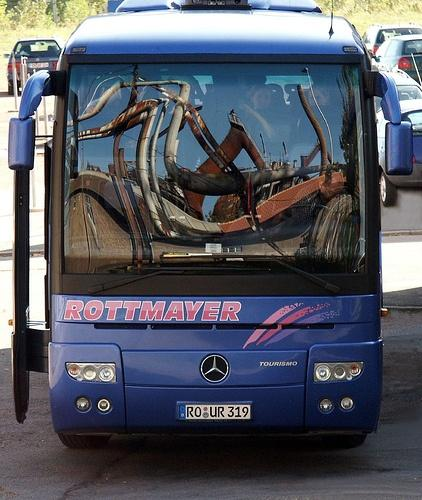
\includegraphics[width=0.11\textwidth]{image/improvement/2007_000663.jpg}
		\enspace\enspace %\hfill
		
\includegraphics[width=0.11\textwidth]{image/improvement/2007_000663.png}
		\enspace\enspace
		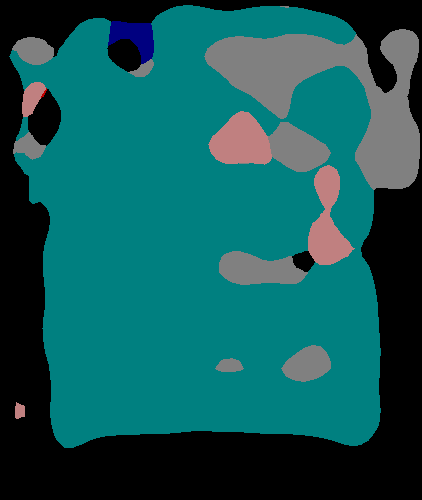
\includegraphics[width=0.11\textwidth]{image/improvement/2007_000663_1.png}
		\enspace\enspace
		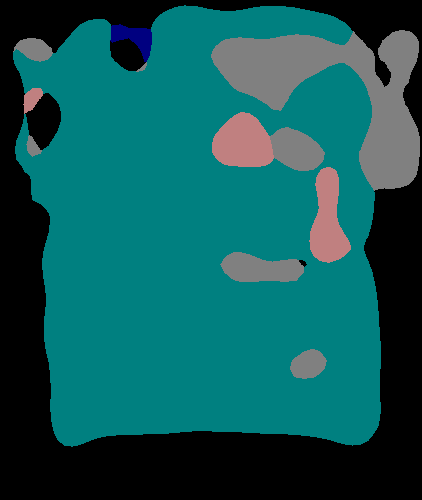
\includegraphics[width=0.11\textwidth]{image/improvement/2007_000663_2.png}
		\enspace\enspace
		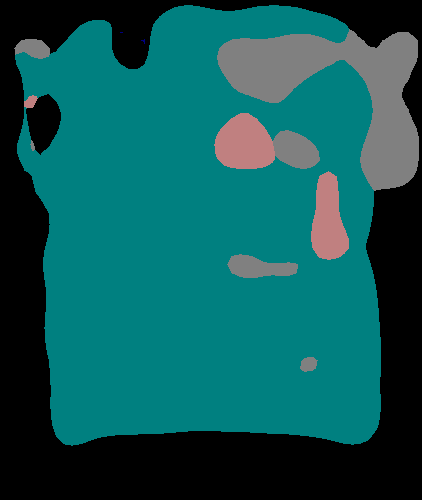
\includegraphics[width=0.11\textwidth]{image/improvement/2007_000663_3.png}
		\enspace\enspace
		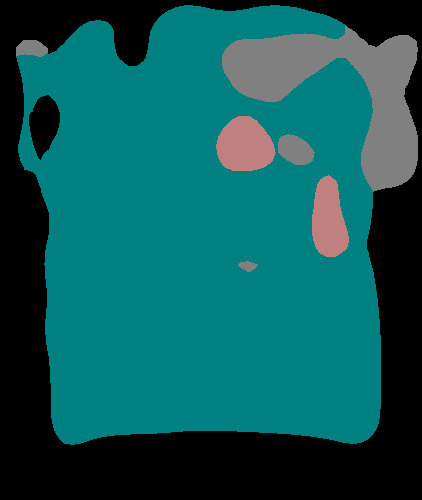
\includegraphics[width=0.11\textwidth]{image/improvement/2007_000663_4.png}
		\enspace\enspace
		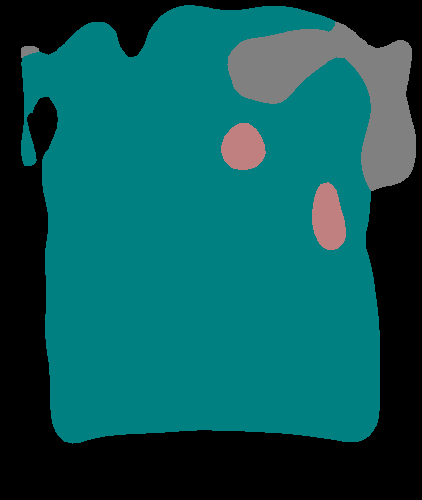
\includegraphics[width=0.11\textwidth]{image/improvement/2007_000663_5.png}
		\enspace\enspace
		\caption[同一网络网格型长短记忆网络时序的增加对输出改善作用的可视化]{网格型长短记忆网络层数增加对输出改善作用的可视化}
		\label{fig:improvement}
	\end{figure}
}

\frame{
   \frametitle{与其它工作的定量对比}
\begin{table}[h] %voc table result
	\centering
		\resizebox{\textwidth}{!}{
		\begin{tabular}{c|*{20}{c}|c}
			\toprule
			Method & aero & bike & bird & boat & bottle & bus & car & cat & chair & cow & table & dog & horse & mbike & person & plant & shep & sofa & train & tv & mIoU.\\
			\midrule
			\midrule
			SDS\footnote{Simultaneous Detection and Segmentation, ECCV 2014}& 63.3 & 25.7 & 63.0 & 39.8 & 59.2 & 70.9 & 61.4 & 54.9 & 16.8 & 45.0 & 48.2 & 50.5 & 51.0 & 57.7 & 63.3 & 31.8 & 58.7 & 31.2 & 55.7 & 48.5 & 51.6 \\
			FCN-8s\footnote{Fully convolutional networks for semantic segmentation, CVPR 2015}  & 76.8 & 34.2 & 68.9 & 49.4 & 60.3 & 75.3 & 74.7 & 77.6 & 21.4 & 62.5 & 46.8 & 71.8 & 63.9 & 76.5 & 73.9 & 45.2 & 72.4 & 37.4 & 70.9 & 55.1 & 62.2\\
			TTI-zoomout-16\footnote{Feedforward semantic segmentation with zoom-out features, CVPR 2015} & \textbf{81.9} & 35.1 & \textbf{78.2} & \textbf{57.4} & 56.5 & 80.5 & 74.0 & 79.8 & 22.4 & 69.6 & 53.7 & 74.0 & \textbf{76.0} & 76.6 & 68.8 & 44.3 & 70.2 & 40.2 & 68.9 & 55.3 &	64.4 \\
			DeepLab-CRF\footnote{Semantic image segmentation with deep convolutional nets and fully connected crfs, ICLR 2015} & 78.4 & 33.1 & \textbf{78.2} & 55.6 & \textbf{65.3} & 81.3 & 75.5 & 78.6 & \textbf{25.3} & 69.2 & 52.7 & \textbf{75.2} & 69.0 & \textbf{79.1} & \textbf{77.6} & \textbf{54.7} & 78.3 & 45.1 & 73.3 & 56.2 & 66.4  \\
			\midrule
			CNN+\textbf{5}LSTM & 80.2 & \textbf{35.3} & 74.1 & 54.4 & 64.4 & \textbf{87.3} & \textbf{81.1} & \textbf{80.6} & 22.7 & \textbf{73.6} & \textbf{58.8} & 73.9 & 73.7 & 78.7 & 77.4 & 50.2 & \textbf{80.0} & \textbf{47.9} & \textbf{76.5} & \textbf{63.1} & \textbf{67.9} \\
			\bottomrule
		\end{tabular}}
		\caption[模型在VOC2012测试集上的结果]{模型在VOC2012测试集上的结果。}		
		\label{tab:voctest}
	\end{table}
	\vspace{-1em}
	\begin{block}{结论}
		\begin{itemize}
			\item[\dag]模型比其他方法有更高的精确度,验证了模型的有效性	
		\end{itemize}
	\end{block}
}
\frame{
   \frametitle{与其它工作的定性对比}
\begin{figure} % image examples & compare
	\begin{subfigure}{0.55\textwidth}
		\centering
		\makebox[0.18\textwidth]{\tiny Grid-5LSTM}
		\makebox[0.18\textwidth]{\tiny FCN-8s}
		\makebox[0.18\textwidth]{\tiny SDS}
		\makebox[0.18\textwidth]{\tiny 真值}
		\makebox[0.18\textwidth]{\tiny 图像} \\
		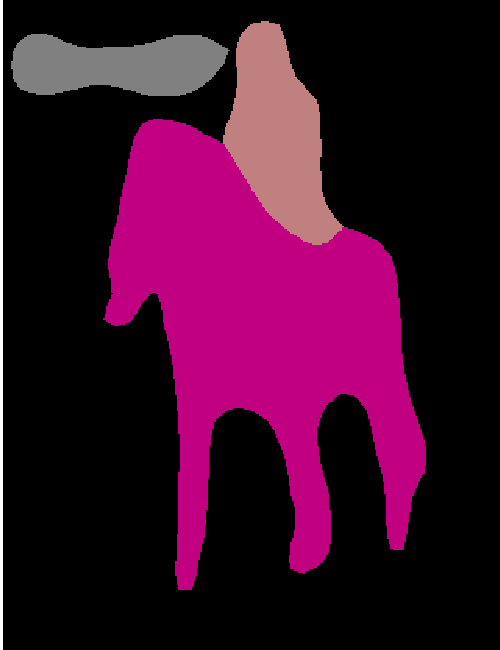
\includegraphics[width=0.18\textwidth]{image/result/compare/my_horse.pdf}
		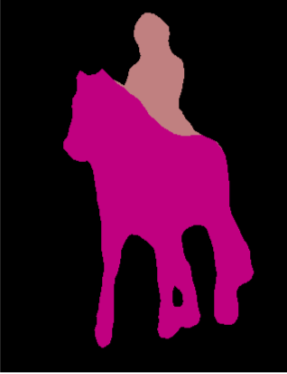
\includegraphics[width=0.18\textwidth]{image/result/compare/fcn_horse.png}
		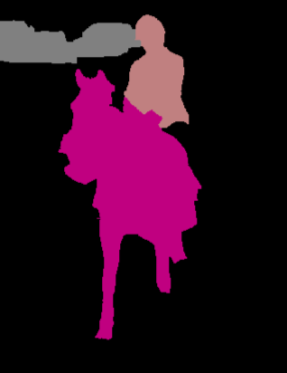
\includegraphics[width=0.18\textwidth]{image/result/compare/sds_horse.png}
		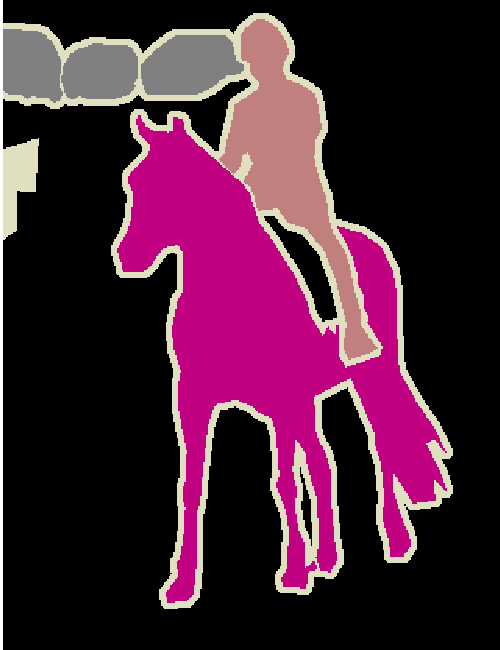
\includegraphics[width=0.18\textwidth]{image/result/compare/gt_horse.pdf}
		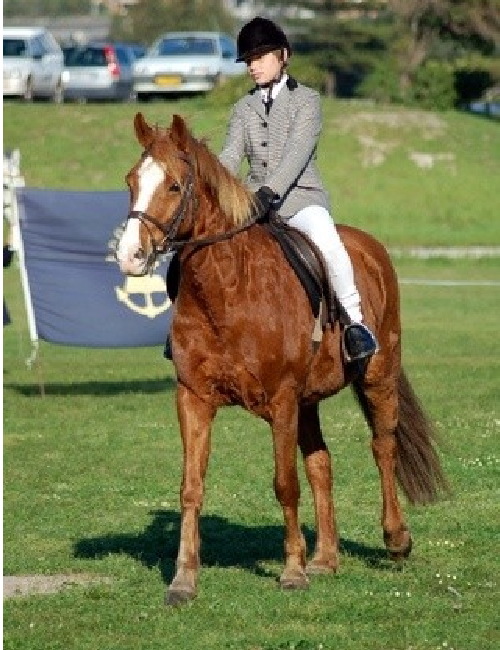
\includegraphics[width=0.18\textwidth]{image/result/compare/im_horse.pdf}
		\\
		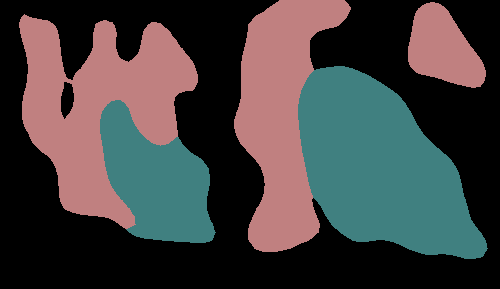
\includegraphics[width=0.18\textwidth]{image/result/compare/my_motor.png}
		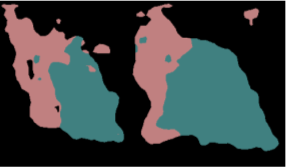
\includegraphics[width=0.18\textwidth]{image/result/compare/fcn_motor.png}
		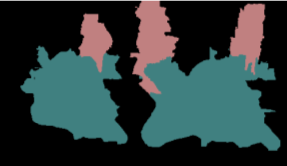
\includegraphics[width=0.18\textwidth]{image/result/compare/sds_motor.png}
		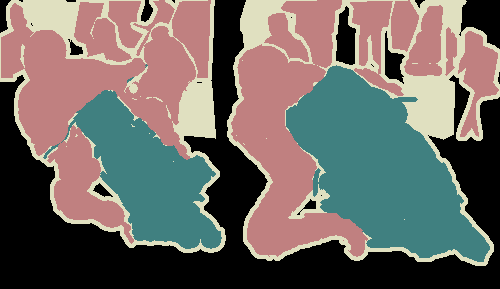
\includegraphics[width=0.18\textwidth]{image/result/compare/2007_005173.png}
		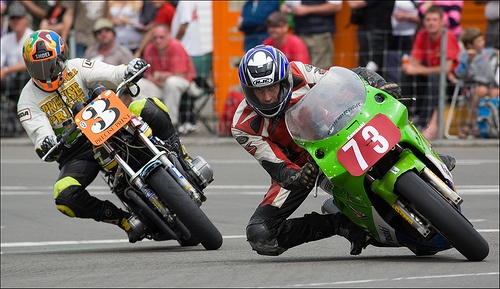
\includegraphics[width=0.18\textwidth]{image/result/compare/2007_005173.jpg}
		\\
		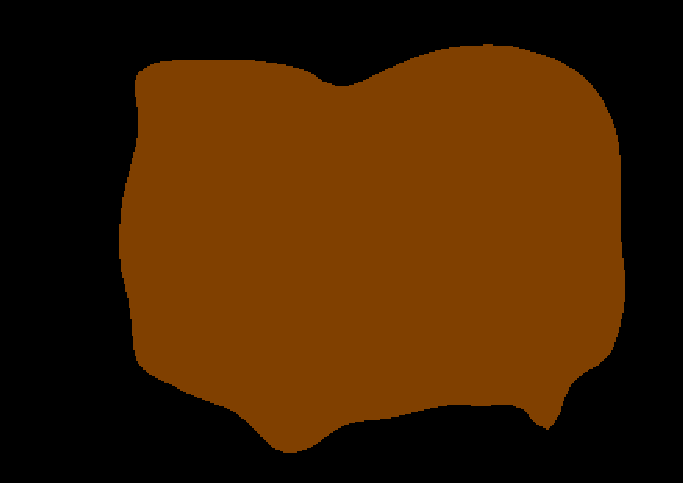
\includegraphics[width=0.18\textwidth]{image/result/compare/my_sheep.pdf}
		
\includegraphics[width=0.18\textwidth]{image/result/compare/fcn_sheep.png}
		
\includegraphics[width=0.18\textwidth]{image/result/compare/sds_sheep.png}
		\includegraphics[width=0.18\textwidth]{image/result/compare/gt_sheep.pdf}
		\includegraphics[width=0.18\textwidth]{image/result/compare/im_sheep.pdf}
		\\
		\includegraphics[width=0.18\textwidth]{image/result/compare/my_boat.png}
		\includegraphics[width=0.18\textwidth]{image/result/compare/fcn_boat.png}
		\includegraphics[width=0.18\textwidth]{image/result/compare/sds_boat.png}
		\includegraphics[width=0.18\textwidth]{image/result/compare/2007_004241.png}
		\includegraphics[width=0.18\textwidth]{image/result/compare/2007_004241.jpg}
		\caption{本文模型效果与其他工作的定性对比}
		\label{fig:compare1}
	\end{subfigure}
	\begin{subfigure}{0.4\textwidth}
		\centering

		\includegraphics[width=0.25\textwidth]{image/result/compare/2010_005284.jpg}
		\includegraphics[width=0.25\textwidth]{image/result/compare/2007_003349.jpg}
		\includegraphics[width=0.25\textwidth]{image/result/compare/2009_004507.jpg} 
		\\
		\includegraphics[width=0.25\textwidth]{image/result/compare/2010_005284.png}
		\includegraphics[width=0.25\textwidth]{image/result/compare/2007_003349.png}
		\includegraphics[width=0.25\textwidth]{image/result/compare/2009_004507.png} \\
		\includegraphics[width=0.25\textwidth]{image/result/compare/zoom_bus.png}
		\includegraphics[width=0.25\textwidth]{image/result/compare/zoom_bird.png}
		\includegraphics[width=0.25\textwidth]{image/result/compare/zoom_dog.png} \\
		\includegraphics[width=0.25\textwidth]{image/result/compare/deeplab_bus.png}
		\includegraphics[width=0.25\textwidth]{image/result/compare/deeplab_bird.png}
		\includegraphics[width=0.25\textwidth]{image/result/compare/deeplab_dog.png} \\
		\includegraphics[width=0.25\textwidth]{image/result/compare/my_bus.png}
		\includegraphics[width=0.25\textwidth]{image/result/compare/my_bird.png}
		\includegraphics[width=0.25\textwidth]{image/result/compare/my_dog.png} 
		\caption{\tiny 其中第一行为图像,第二行为真值,第三行为TTI-zoomout-16,第四行为DeepLab-CRF,第五行是Grid-5LSTM的结果}
		\label{fig:compare2}
	\end{subfigure}
	\caption{Grid-5LSTM与其它模型在VOC 2012验证集上的定性比较}
	\end{figure}
}

\frame{
   \frametitle{一些分割失败的例子}
	\begin{figure}[h]
		\centering
		\makebox[0.15\textwidth]{\footnotesize 图像}
		\makebox[0.15\textwidth]{\footnotesize 真值}
		\makebox[0.15\textwidth]{\tiny CNN+5LSTM}
		\quad
		\makebox[0.15\textwidth]{\footnotesize 图像} 
		\makebox[0.15\textwidth]{\footnotesize 真值}
		\makebox[0.15\textwidth]{\tiny CNN+5LSTM}\\
		\includegraphics[width=0.15\textwidth]{image/result/error/2008_000673.jpg}
		\includegraphics[width=0.15\textwidth]{image/result/error/2008_000673.png}
		\includegraphics[width=0.15\textwidth]{image/result/error/p_2008_000673.png} 
		\quad
		\includegraphics[width=0.15\textwidth]{image/result/error/2008_001580.jpg} 
		\includegraphics[width=0.15\textwidth]{image/result/error/2008_001580.png}
		\includegraphics[width=0.15\textwidth]{image/result/error/p_2008_001580.png} 
		\\
		\includegraphics[width=0.15\textwidth]{image/result/error/2007_002539.jpg}
		\includegraphics[width=0.15\textwidth]{image/result/error/2007_002539.png}
		\includegraphics[width=0.15\textwidth]{image/result/error/p_2007_002539.png}
		\quad
		\includegraphics[width=0.15\textwidth]{image/result/error/2007_008964.jpg}
		\includegraphics[width=0.15\textwidth]{image/result/error/2007_008964.png}
		\includegraphics[width=0.15\textwidth]{image/result/error/p_2007_008964.png}
		\\
		\includegraphics[width=0.15\textwidth]{image/result/error/2008_000763.jpg}
		\includegraphics[width=0.15\textwidth]{image/result/error/2008_000763.png}
		\includegraphics[width=0.15\textwidth]{image/result/error/p_2008_000763.png}
		\quad
		\includegraphics[width=0.15\textwidth]{image/result/error/2007_009088.jpg}
		\includegraphics[width=0.15\textwidth]{image/result/error/2007_009088.png}
		\includegraphics[width=0.15\textwidth]{image/result/error/p_2007_009088.png}
		\\
	\color[rgb]{0.9,0.9,0.9}\bfseries
	\resizebox{\textwidth}{!}{
	\begin{tabular}{*{7}{>{\centering\arraybackslash}p{0.111\textwidth}}}
		\hline
		\cellcolor[rgb]{0,0,0}  背景&\cellcolor[rgb]{0.5020,0,0} 飞机 &\cellcolor[rgb]{0,0.5020,0} 自行车 &\cellcolor[rgb]{0.5020,0.5020,0} 鸟 &\cellcolor[rgb]{0,0,0.5020} 船   &\cellcolor[rgb]{0.5020,0,0.5020} 瓶子 &\cellcolor[rgb]{0,0.5020,0.5020} 大巴
		\\
		\hline
		\cellcolor[rgb]{0.5020,0.5020,0.5020} 汽车 & \cellcolor[rgb]{0.2510,0,0} 猫 &\cellcolor[rgb]{0.7529,0,0} 椅子 &\cellcolor[rgb]{0.2510,0.5020,0} 牛 &\cellcolor[rgb]{0.7529,0.5020,0} 桌子 &\cellcolor[rgb]{0.2510,0,0.5020} 狗 &\cellcolor[rgb]{0.7529,0,0.5020} 马 \\
		\hline
		\cellcolor[rgb]{0.2510,0.5020,0.5020} 摩托车 &\cellcolor[rgb]{0.7529,0.5020,0.5020} 人   &\cellcolor[rgb]{0,0.2510,0} 盆栽   &\cellcolor[rgb]{0.5020,0.2510,0} 羊 &\cellcolor[rgb]{0,0.7529,0} 沙发 &\cellcolor[rgb]{0.5020,0.7529,0} 火车 &\cellcolor[rgb]{0,0.2510,0.5020} 电视 \\
		\hline
	\end{tabular}
	}
	\caption[一些模型分类错误的例子]{一些CNN+5LSTM分类错误的例子}
		\label{fig:error}
	\end{figure}
}

\subsection*{SIFT FLOW实验结果}
\frame{
   \frametitle{SIFT FLOW实验结果}
\begin{table}[h] %voc table result
	\centering
		\resizebox{0.8\textwidth}{!}{
		\begin{tabular}{*{4}{c}}
			\toprule
	 		Method & Pixel Acc. & Mean Acc. & Mean IU.\\
			\midrule
			Liu et al.\footnote{Sift flow: Dense correspondence across scenes and its applications, PAMI 2011}   & 76.7 & - & -\\
			Tighe et al.\footnote{Finding things: Image parsing with regions and per-exemplar detectors, CVPR 2013} & 78.6 & 39.2 & -\\
			FCN-16s\footnote{Fully convolutional networks for semantic segmentation, CVPR 2015} & 85.2 & \textbf{51.7} & 39.5\\
			Deeplab-LargeFOV\footnote{emantic image segmentation with deep convolutional nets and fully connected crfs, ICLR 2015}& 85.6 & 51.2 & 39.7\\
			\midrule
			Grid-5LSTM & \textbf{86.2} & 51.0 & \textbf{41.2}\\
			\bottomrule
		\end{tabular}
	}
		\caption[模型在SIFT FLOW上的结果]{模型在SIFT FLOW上的结果。Tighe等人的方法是用SVM+MRF,Deeplab-LargeFOV的结果是通过公开的源码实验得到的}		
		\label{tab:siftflow}
	\end{table}
}

\endinput

\section{总结与展望}
\subsection*{总结与展望}
\frame{
   \footnotesize
	\begin{block}{工作总结}
	\begin{itemize}
		\item[\dag] 本文的模型结合了卷积网络的特征学习能力与长短记忆网络对整体局部建模的能力,相比于全卷积网络,大幅度地提高了了模型性能
		\item[\dag] 大量的对比实验与结果分析证明了模型的有效性 
	\end{itemize}
	\end{block}
	\vspace{-1em}
	\begin{block}{展望}
	\begin{itemize}
		\item[\dag] 模型性能:提高网络的深度来学习更高层次的特征,提高模型效果(He et al. ResNet, CVPR 2016)
		\item[\dag] 模型大小:通过裁剪网络冗余部分(Han et al. Deep Compression, ICLR 2016 Best Paper)或使用二值网络减少模型参数(Courbariaux et al. Binaryconnect, NIPS 2015)
		\item[\dag] 训练数据:使用无监督或弱监督的方式训练网络(Papandreou et al. Weakly-and semi-supervised learning, ICCV 2015)
	\end{itemize}
	\end{block}
}



\section{致谢}
\subsection*{致谢}
\frame{
	\frametitle{致谢}
	\begin{block}{感谢每一个帮助过我的人}
	\begin{itemize}
		\item 首先要感谢的是我的指导老师的悉心指导
		\item 感谢师兄师姐、同学的帮助
		\item 感谢家人的支持
		\item 感谢答辩委员会的聆听和指导
	\end{itemize}
	\end{block}
	\vspace{-1em}
	\note{
		我的展示到此结束,我要感谢我的指导老师,师兄师姐同学,家人还有答辩委员会老师的聆听与指导。谢谢大家
	}
}
\frame{
	\frametitle{Q \& A}
	\begin{block}{Questions?}
	 ~\\ ~\\
	 \center{\Large{Thank you!}}
	 \\ ~\\ ~\\ ~\\ ~\\ 
	\end{block}
	\note{
		现在是问答时间。请问老师们对我的展示有什么疑问?
	}
}



\end{document}
